\subsection{Existierender Data-Lake-Prototyp}
In einem Masterprojekt an der Hochschule Niederrhein \parencite{prototyp} wurde ein Prototyp für ein Data-Lake-System entwickelt.
In \cref{fig:prototyp-architektur} ist ein Überblick über dessen Architektur zu sehen.
Es handelt sich hierbei um eine Client-Server-Anwendung.
Der Client besteht aus einer Web-Anwendung über die Benutzer mit dem Data-Lake-System interagieren.
Er kommuniziert mit dem Server über eine REST-API, die auch durch andere Clients verwendet werden könnte.
Die Datenverarbeitung wird über ein Spark-Cluster gelöst.
Zum Speichern der Daten stehen drei verschiedene System zu Verfügung.
Es kommen eine PostgreSQL Datenbank für strukturierte, eine MongoDB für semistrukturierte und ein HDFS für unstrukturierte Daten zum Einsatz.

\begin{figure}
    \centering
    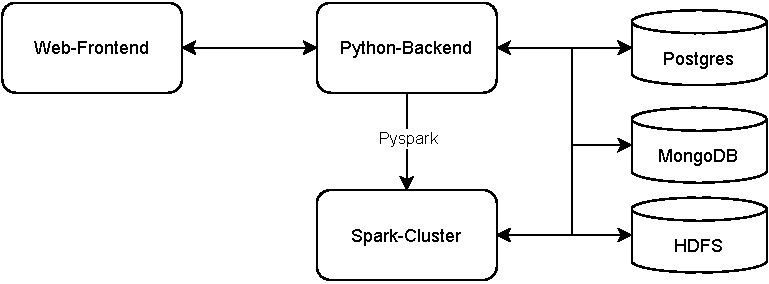
\includegraphics{Grafiken/Prototyp-Architektur.pdf}
    \caption[Architektur des Prototyp]{Architektur des Prototyp}
    \label{fig:prototyp-architektur}
\end{figure}

Die Verarbeitung der Ingestion ist im Prototyp abhängig von der Datenquelle und dem ausgewählten Zielspeicher.
In \cref{fig:prototyp-ingestion}  sind die verschiedenen Wege zu sehen.
Diese Verarbeitungsweise hat zwei Probleme, die in der neuen Ingestion gelöst werden müssen.
Dadurch, dass der Benutzer aus den verschiedenen Speichern ein Ziel auswählt, können hier leicht Probleme entstehen, falls die Datenquelle nicht mit dem Format des Speichers kompatibel ist.
Außerdem sind die Verarbeitungen der Quellen zu den Speichern fest im Code des Servers einprogrammiert.
So ist es nicht möglich während der Laufzeit neue Datenquellen zu integrieren.

\begin{figure}
    \centering
    \subfigure[Datenbank-Ingestion]{
        \label{fig:prototyp-db-ingeston}
        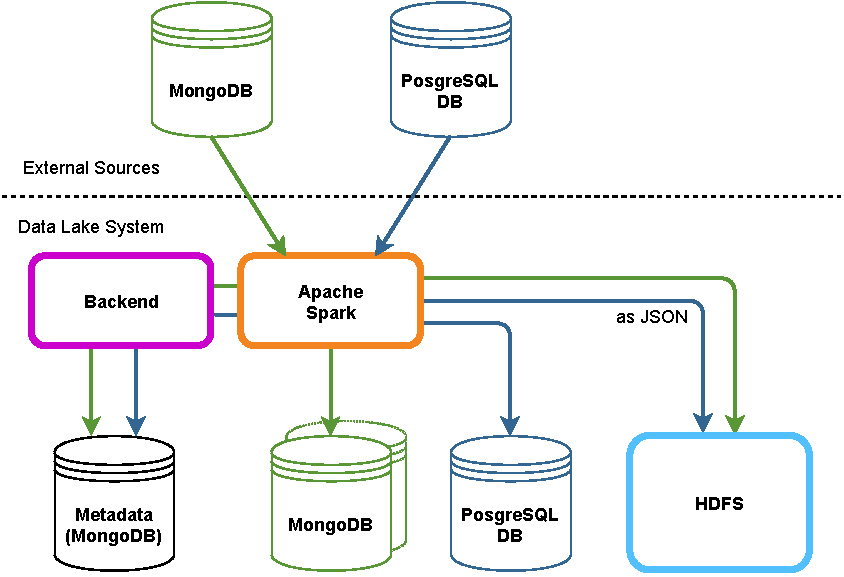
\includegraphics[width=.45\textwidth]{Grafiken/db_ingestion.pdf}
    }
    \subfigure[Datei-Ingestion]{
        \label{fig:prototyp-file-ingeston}
        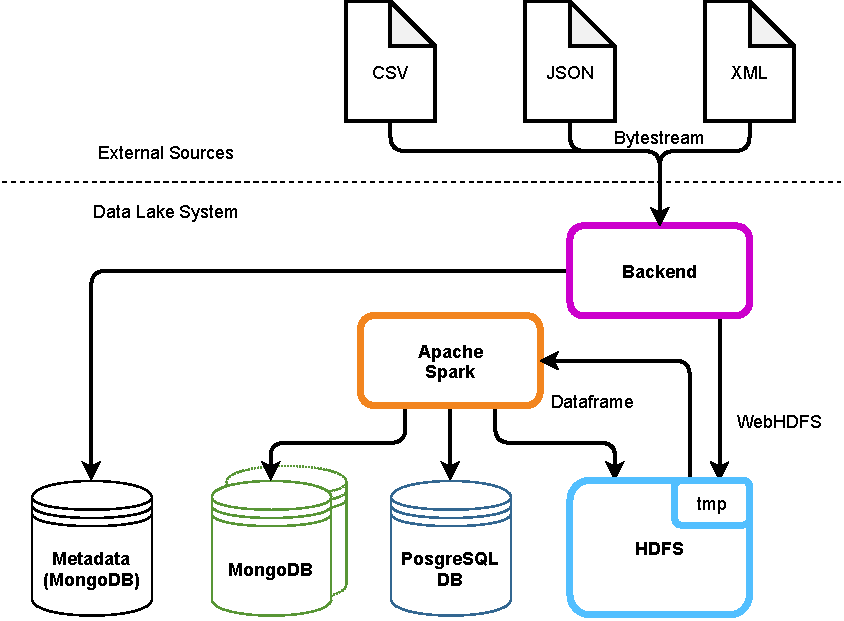
\includegraphics[width=.45\textwidth]{Grafiken/file_ingestion.pdf}
    }
    \caption[Ingestion-Verarbeitung des Prototyp]{Ingestion-Verarbeitung des Prototyp, \citetitle[Quelle:][S. 3]{prototyp}}
    \label{fig:prototyp-ingestion}
\end{figure}

Im Vorlauf dieser Arbeit wurde ein Refactoring des Prototyp durchgeführt.
Dabei wurde festgestellt, dass die Erweiterung des Data-Lake-Systems um die Kompatibilität mit weiteren Datenquellen ein aufwändiger Prozess ist.
Auch durch die gewählten Speichersysteme für die geladenen Daten erschweren die Integration einer Lösung für die Versionierung der Daten.
Daher wurde beschlossen, dass eine dedizierte Ingestion-Schnittstelle für das System entwickelt werden soll.